% !TEX program = xelatex
\documentclass[a4paper]{article}
\usepackage[UTF8]{ctex}
\setCJKmainfont{SimSun}[BoldFont=SimHei,ItalicFont=KaiTi]
\setCJKsansfont{SimHei}
\usepackage[top=3mm,bottom=3mm,left=3mm,right=3mm]{geometry}
\usepackage{amsmath,amssymb,bm}
\usepackage{multicol}
\usepackage{tikz}
\usetikzlibrary{arrows.meta,calc}
\usepackage[dvipsnames]{xcolor}
\usepackage{array,tabularx}
\pagestyle{empty}
\setlength{\parindent}{0pt}
\setlength{\parskip}{0pt}
\setlength{\columnsep}{2.0mm}
\setlength{\columnseprule}{0.12pt}
\setlength{\tabcolsep}{1.0pt}
\setlength{\fboxsep}{0.65pt}
\renewcommand{\baselinestretch}{0.66}
\definecolor{h}{HTML}{0B3D91}
\definecolor{b}{HTML}{1565C0}
\definecolor{r}{HTML}{B71C1C}
\definecolor{o}{HTML}{E65100}
\definecolor{g}{HTML}{1B5E20}
\definecolor{bg}{HTML}{EEF3FF}
\definecolor{warnbg}{HTML}{FFF2E6}
\definecolor{grid}{HTML}{D6DEE8}
\newsavebox{\fitbox}
\newcommand{\fitmath}[2][\dimexpr\linewidth-4pt\relax]{\sbox{\fitbox}{$\displaystyle #2$}\ifdim\wd\fitbox>#1\resizebox{#1}{!}{$\displaystyle #2$}\else\usebox{\fitbox}\fi}
\newcommand{\E}[1]{\colorbox{bg}{\fitmath{#1}}}
\newcommand{\Hh}[1]{\vspace{0.35pt}{\fontsize{6.1}{6.25}\selectfont\bfseries\color{white}\colorbox{h}{\strut\ #1\ }}\par\vspace{0.2pt}}
\newcommand{\linea}[2]{\textbf{\color{b}#1}：#2\par}
\newcommand{\warn}[1]{\colorbox{warnbg}{\begin{minipage}{\dimexpr\linewidth-2\fboxsep\relax}\fontsize{4.72}{4.95}\selectfont\textbf{\color{r}错}：#1\end{minipage}}\par}
\newcommand{\modu}[5]{\vspace{0.35pt}\noindent\fcolorbox{grid}{white}{\begin{minipage}{0.976\linewidth}\fontsize{4.72}{4.95}\selectfont\textbf{\color{h}#1}\par\linea{题干}{#2}\linea{第一行}{#3}\linea{公式链}{#4}\linea{扩展/简答/错}{#5}\end{minipage}}\par}
\newcommand{\mini}[2]{\vspace{0.25pt}\noindent\fcolorbox{grid}{white}{\begin{minipage}{0.976\linewidth}\fontsize{4.72}{4.95}\selectfont\textbf{\color{h}#1}\par #2\end{minipage}}\par}
\newcommand{\formula}[2]{\mini{#1}{\colorbox{bg}{\begin{minipage}{\dimexpr\linewidth-2\fboxsep\relax}\centering\fontsize{4.55}{4.75}\selectfont #2\end{minipage}}}}
\newcommand{\pipeicon}{\begin{center}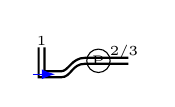
\begin{tikzpicture}[>=Latex,scale=.38,every node/.style={font=\tiny}]
\draw[thick](0,1)--(0,0)--(.75,0)..controls(1.1,0)and(1.1,.45)..(1.55,.45)--(3.0,.45);
\draw[thick](.2,1)--(.2,.2)--(.75,.2)..controls(1.0,.2)and(1.1,.65)..(1.55,.65)--(3.0,.65);
\draw[->,blue](-.2,.1)--(.55,.1);\node[circle,draw,inner sep=1pt] at (2.0,.55){P};\node at(.1,1.2){1};\node at(2.85,.85){2/3};
\end{tikzpicture}\end{center}}
\newcommand{\lavalicon}{\begin{center}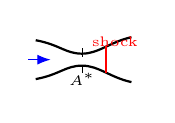
\begin{tikzpicture}[>=Latex,scale=.38,every node/.style={font=\tiny}]
\draw[thick](0,.65)..controls(.8,.5)and(1.0,.2)..(1.55,.2)..controls(2.1,.2)and(2.5,.6)..(3.2,.75);
\draw[thick](0,-.65)..controls(.8,-.5)and(1.0,-.2)..(1.55,-.2)..controls(2.1,-.2)and(2.5,-.6)..(3.2,-.75);
\draw[dashed](1.55,-.45)--(1.55,.45);\node at(1.55,-.65){$A^*$};\draw[->,blue](-.25,0)--(.5,0);\draw[red,thick](2.35,-.45)--(2.35,.45);\node[red]at(2.65,.6){shock};
\end{tikzpicture}\end{center}}
\newcommand{\cvicon}{\begin{center}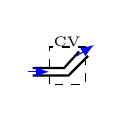
\begin{tikzpicture}[>=Latex,scale=.38,every node/.style={font=\tiny}]
\draw[thick](0,.3)--(1.2,.3)--(1.85,.95);\draw[thick](0,.55)--(1.05,.55)--(1.55,1.1);\draw[dashed](.55,.0)rectangle(1.75,1.25);
\draw[->,blue](-.15,.42)--(.55,.42);\draw[->,blue](1.47,.95)--(2.05,1.32);\node at(1.15,1.43){CV};
\end{tikzpicture}\end{center}}
\newcommand{\poticon}{\begin{center}\begin{tikzpicture}[>=Latex,scale=.36,every node/.style={font=\tiny}]
\foreach \y in{-.35,0,.35}{\draw[->,blue](-.1,\y)--(.8,\y);}\draw[thick](1.15,0)circle(.32);\node at(1.15,-.55){圆柱};
\draw[fill=black](2.1,0)circle(.04);\node[above]at(2.1,0){源};\draw[thick](2.75,-.5)..controls(3.2,-.75)and(3.6,-.75)..(4.0,-.5);
\end{tikzpicture}\end{center}}
\newcommand{\stressicon}{\begin{center}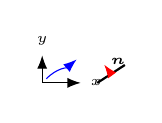
\begin{tikzpicture}[>=Latex,scale=.35,every node/.style={font=\tiny}]
\draw[->](0,0)--(1.4,0)node[right]{$x$};\draw[->](0,0)--(0,1.0)node[above]{$y$};\draw[blue,->](.15,.15)..controls(.55,.55)and(.9,.55)..(1.25,.85);
\draw[thick](2.0,0)--(3,.65);\draw[->,red](2.5,.32)--(2.25,.66);\node at(2.75,.77){$\bm n$};
\end{tikzpicture}\end{center}}

\begin{document}
\fontsize{4.82}{5.00}\selectfont

% ================= PAGE 1 =================
\begin{multicols}{3}
\Hh{P1 母题1：管路/泵/水轮机/汽蚀}
\mini{15秒定位}{先看题干图形：水池/管/泵$\to$A；静水/U管$\to$B；弯管/喷流$\to$C；源汇涡/圆柱$\to$D；$Ma,p_0,T_0,A^*,p_b$/激波$\to$E；$Re,\mu,\tau_w,\delta,C_D\to$F；速度场/应力/量纲/证明$\to$G。}
\mini{固定首句}{取\_\_为研究对象，设1为\_\_，2为\_\_，取\_\_为正，在\_\_假设下列\_\_方程。最后必须写单位、方向、表压/绝压、查表入口。}
\formula{通用量}{\(\displaystyle Q=AV,\quad \dot m=\rho Q,\quad Re=\frac{VL}{\nu}=\frac{\rho VL}{\mu},\quad Ma=\frac{V}{\sqrt{\gamma RT}}\)}
\pipeicon
\modu{母题1 主模板：管路机械能}{水池、长管、泵、阀、弯头、压力表、粗糙度}{画1,2,3截面；液面/自由射流常取表压0}{\(V_i=Q/A_i\to Re_i\to \lambda_i\to h_L\to\)修正Bernoulli}{局部损失用所在管径速度；效率位置别反；粗糙度用于\(\epsilon/d\)}
\formula{母题1核心式：机械能}{\(\displaystyle z_1+\frac{p_1}{\rho g}+\frac{\alpha_1V_1^2}{2g}+H_p=z_2+\frac{p_2}{\rho g}+\frac{\alpha_2V_2^2}{2g}+H_T+h_f+h_\zeta\)}
\modu{母题1扩展A：水池到出口求Q}{水池接长管、出口大气、求流量}{1水面2出口，\(p_1=p_2=0,V_1\approx0\)}{\(H=(1+\lambda L/d+\sum\zeta)V^2/2g,\ Q=AV\)}{若\(\lambda\)随Re变，先估再迭代；不要漏出口速度头}
\modu{母题1扩展B：泵/水轮机功率}{泵、扬程、轴功率、效率、输水}{列能量解\(H_p\)或\(H_T\)}{泵给流体：\(P_w=\rho gQH_p\)；轴功率：\(P_s=\rho gQH_p/\eta\)}{水轮机取能：输出\(P=\eta\rho gQH_T\)}
\modu{母题1扩展C：汽蚀/安装高度}{泵高于水面、汽化压、入口压至少高于}{从水面1到泵入口2列能量}{\(p_2=p_a-\rho g(z_2-z_1)-\rho V^2/2-\rho gh_L\ge p_v+\Delta p\)}{汽化压必须绝压；吸入段阀/弯头都算损失}
\modu{母题1扩展D：多管径/串并联}{内径改变、串联、并联、分流}{每段单独定义\(V_i,Q_i,Re_i\)}{串联同Q损失相加；并联同端点\(h_{La}=h_{Lb}\), \(Q=Q_a+Q_b\)}{不同管径不能共用一个速度}
\modu{母题1扩展E：粗糙度/Moody}{镀锌钢管、铸铁、粗糙度、压降反推}{先算\(Re,\epsilon/d\)}{已知\(Q\)查\(\lambda\)；已知压降先由能量解\(\lambda\)，再反查\(\epsilon/d\)}{层流\(\lambda=64/Re\)，不用Moody}
\modu{母题1扩展F：文丘里/孔口/喷嘴}{差压计、孔口、喷嘴、流量测量}{1上游2喉/孔口，写Bernoulli+连续}{理想文丘里：\(Q=A_2\sqrt{2\Delta p/[\rho(1-(A_2/A_1)^2)]}\)；实际乘\(C_d\)}{孔口出流常\(Q=C_dA\sqrt{2gH}\)}
\modu{母题1扩展G：局部损失}{入口、阀门、弯头、突然扩大/缩小}{把局部件放进\(\sum\zeta V^2/2g\)}{突然扩大可用\((V_1-V_2)^2/2g\)}{局部损失不是粗糙度；速度取局部件所在截面}
\mini{母题1改皮A：水池到水池}{1、3都是大水面：\(p_1=p_3=0\)表压，\(V_1,V_3\approx0\)。能量方程变成“水位差 = 沿程 + 局部 + 泵/水轮机”。若求\(Q\)，损失全写成\(KQ^2\)。}
\mini{母题1改皮B：泵吸水安装高度}{1水面，2泵入口：\(p_2=p_a-\rho g(z_2-z_1)-\rho V^2/2-\rho gh_L\)。约束 \(p_2\ge p_v+\Delta p_{safe}\)，求最大\(h=z_2-z_1\)。}
\mini{母题1改皮C：水轮机输出}{上游到下游列能量，水轮机头\(H_T\)是被取走的能量。轴功率 \(P=\eta\rho gQH_T\)。若题问水流给转轮功率，先不乘效率。}
\mini{母题1改皮D：反推粗糙度}{已知实际\(Q\)：先算\(V,Re\)，由能量式解\(\lambda\)，再查Moody得\(\epsilon/d\)。不要用光滑湍流公式反推粗糙度。}
\mini{母题1改皮E：串并联系统}{串联同\(Q\)，各段损失相加；并联同端点总水头损失相等，\(h_{La}=h_{Lb}\)，且 \(Q=Q_a+Q_b\)。每支路独立算\(V,Re,\lambda\)。}
\mini{母题1填空/简答}{局部阻力系数\(\zeta\)不是摩阻系数\(\lambda\)；粗糙度只通过\(\epsilon/d\)进Moody；水泵给流体加机械能，水轮机从流体取机械能。}
\mini{母题1必检}{\(m^3/h\)先除3600；直径mm先转m；自由液面/自由射流常取表压0；普通管路算出MPa级压强时先查单位和水头。}
\mini{母题1弱化1：给水位差求\(Q\)}{设\(V=Q/A\)，写 \(H=V^2/2g+\lambda(L/d)V^2/2g+\sum\zeta V^2/2g\)。若\(\lambda\)随Re变，先估再迭代。}
\mini{母题1弱化2：给\(Q\)求入口压}{吸入段已知\(Q\)时，先算\(V,Re,\lambda,h_L\)，再用 \(p_{in}=p_a-\rho gh-\rho V^2/2-\rho gh_L\)。}
\mini{母题1弱化3：压力表求泵功}{压力表读数直接进 \(p/\rho g\) 表压项；先解\(H_p\)，再判题问水功率还是轴功率：轴功率除以\(\eta\)。}
\mini{母题1弱化4：局部突然扩大}{优先写 \(h=(V_1-V_2)^2/(2g)\)。若题给\(\zeta\)，按题指定速度头；没指定通常用局部件所在截面速度。}
\mini{母题1弱化5：流量测量}{文丘里/喷嘴用Bernoulli+连续，孔口出流常用 \(Q=C_dA\sqrt{2gH}\)。差压计给的是\(\Delta p\)，先转成压强差。}
\mini{母题1弱化6：效率题}{泵：流体获得功率 \(P_w=\rho gQH_p\)，轴输入 \(P_s=P_w/\eta\)。水轮机：轴输出 \(P_s=\eta\rho gQH_T\)。}
\mini{母题1弱化7：多出口/支路}{节点连续 \(\sum Q_{in}=\sum Q_{out}\)。并联不加损失，只令两支路端点水头损失相等。}
\mini{母题1弱化8：粗糙题}{题干“镀锌/铸铁/粗糙度\(h\)”先算\(\epsilon/d\)，再与\(Re\)查Moody。题给\(\lambda\)就不用再查。}
\mini{母题1截面编号}{水池到管口：1水面、2管口；泵题：1吸入水面、2泵入口、3泵出口；压力表题：压力表所在位置单独设截面。}
\mini{母题1压强式写法}{也可用压力形式：\(p_1+\rho gz_1+\frac12\rho V_1^2+\Delta p_p=p_2+\rho gz_2+\frac12\rho V_2^2+\Delta p_L\)。}
\mini{母题1高度差}{图上“泵中心高于水面\(h\)”就是 \(z_2-z_1=h\)。沿斜管长度不是竖直高度，竖直高度只读标高差。}
\mini{母题1迭代写法}{若\(\lambda\)未知：先假设\(\lambda\)或光滑湍流，解\(Q\)，算\(Re\)，查新\(\lambda\)，重复到变化小。写出这个流程可拿过程分。}
\mini{母题1真空/表压}{真空表读数常表示表压为负；能量式若全用表压，大气相通点取0；汽蚀比较必须换绝压。}
\mini{母题1局部件速度}{入口损失常用管内速度；阀门/弯头用所在管段速度；突然扩大若不用\(\zeta\)，用\((V_1-V_2)^2/2g\)。}
\mini{母题1结果自检}{水泵扬程应为正；水轮机头应为可取出的能量；损失项永远非负；若流动方向反了，速度符号或高程方向要重设。}
\mini{母题1大题骨架}{第一行：取1为上游水面，2为机器入口/测压点，3为出口。第二行：\(Q\to V_i\to Re_i\to\lambda_i\)。第三行：列机械能方程解目标量。}
\mini{母题1求流量完整链}{未知 \(Q\) 时，把所有速度写成 \(V_i=Q/A_i\)，所有损失写成 \(K_iQ^2\)。若 \(\lambda\) 也未知，写“试算 \(Q\)-更新 \(Re,\lambda\)-迭代”。}
\mini{母题1求压力完整链}{已知 \(Q\) 求某点压力：先算各段 \(V,Re,\lambda,h_L\)，从已知压力截面列到未知截面，最后解 \(p\)。压力表通常给表压。}
\mini{母题1求泵扬程}{泵在方程中加能量 \(+H_p\)。若题给轴功率 \(P_s\)，则 \(H_p=\eta P_s/(\rho gQ)\)。若求轴功率，\(P_s=\rho gQH_p/\eta\)。}
\mini{母题1求水轮机}{水轮机从水流取能，方程右侧可写 \(+H_T\) 或左侧写 \(-H_T\)。输出轴功率 \(P_s=\eta\rho gQH_T\)。}
\mini{母题1求安装高度}{水面1到泵入口2：\(p_2=p_a-\rho gh-\rho V^2/2-\rho gh_L\)。令 \(p_2\ge p_v+\Delta p\)，解最大 \(h\)。}
\mini{母题1粗糙度反推}{已知压降和流量：能量式先解 \(\lambda\)，再由 \(Re,\lambda\) 到Moody图反查 \(\epsilon/d\)，最后 \(\epsilon=d(\epsilon/d)\)。}
\mini{母题1并联联立}{并联两支路同端点，因此 \(h_{La}=h_{Lb}\)，且 \(Q=Q_a+Q_b\)。若两管不同，设 \(Q_a,Q_b\) 分别算 \(V,Re,\lambda\)。}
\mini{母题1串联分段}{串联同一流量 \(Q\)，不同管径速度不同，损失逐段相加：\(\sum \lambda_i(L_i/d_i)V_i^2/(2g)+\sum\zeta_iV_i^2/(2g)\)。}
\mini{母题1突然扩大/缩小}{突然扩大优先 \(h=(V_1-V_2)^2/(2g)\)。突然缩小若题给 \(\zeta\)，按指定截面速度头；未给则用教材表。}
\mini{母题1入口出口}{水池入口到管内常有入口损失；管口自由出流要保留出口速度头 \(V^2/2g\)。两个大水池相连时两端水面速度可忽略。}
\mini{母题1差压计测流}{文丘里/孔板：先由差压计换 \(\Delta p\)，再用Bernoulli+连续。实际流量常乘流量系数 \(C_d\)。}
\mini{母题1压力线}{能量线沿程因损失下降，经过泵上跳，经过水轮机下跳。若画线题，局部损失处有突降，沿程损失为斜降。}
\mini{母题1水头单位}{\(p/\rho g\) 单位是m水柱；\(V^2/2g\) 是速度水头；\(h_f,h_\zeta,H_p,H_T\) 都是水头。不要把Pa直接和m相加。}
\mini{母题1层流特例}{若 \(Re<2300\)，直接 \(\lambda=64/Re\)，不查Moody。层流沿程损失与平均速度一次方等价，湍流近似与速度平方相关。}
\mini{母题1光滑湍流估算}{若题写光滑管且无Moody图，可用Blasius近似 \(\lambda=0.3164/Re^{1/4}\)（常见适用范围按教材）。}
\mini{母题1压力表位置}{压力表接在管中心线处，\(z\) 取该点标高；若表在管顶/管底且题强调位置，需加上管内竖向高度差。}
\mini{母题1水箱液面}{大水箱自由面：表压0，速度约0。若水箱封闭或液面上有气压，则 \(p/\rho g\) 不能取0。}
\mini{母题1能量方程移项}{建议永远把未知量单独留一边：求 \(H_p\) 时把损失和下游项移到右边；求 \(p_2\) 时把其他项移开，避免符号错。}
\mini{母题1泵/水轮机方向}{泵使总水头增加，水轮机使总水头减少。若算出泵扬程为负，说明实际不是泵加能，或截面方向设反。}
\mini{母题1常见关键词}{“水温/运动粘度”提示算 \(Re\)；“粗糙度”提示Moody；“弯头/阀门”提示局部损失；“汽化压”提示绝压。}
\mini{母题1最后一句模板}{故所求 \(Q=\_\_\,m^3/s\)；或 \(p=\_\_\,kPa\)（表压/绝压）；或泵轴功率 \(P_s=\_\_\,kW\)。损失项均已计入。}
\end{multicols}
\newpage

% ================= PAGE 2 =================
\begin{multicols}{3}
\Hh{P2 母题2-4：静水 / 动量 / 势流}
\modu{母题2 主模板：静水压强受力}{静止液体、水面、U管、闸门、浮体}{先写\(p=p_0+\rho gh\)，\(h\)是竖直深度}{受力：找形心深度\(h_c\)、合力\(F\)、压力中心/力矩}{填空：静水压强只随竖直深度变；斜板长度不是水头}
\modu{母题2扩展A：U管/差压计}{U形管、水银、两点压差}{沿液柱走：向下加\(\rho gh\)，向上减}{同一静止连通液体同高压强相等}{最后按题问表压/绝压；水银密度别当水}
\modu{母题2扩展B：平面闸门}{矩形/圆形闸门、铰链、开启力}{\(F=\rho gh_cA\)}{\(h_p=h_c+I_G/(h_cA)\)，再对铰链取矩}{合力不在形心；倾斜面仍用竖直深度}
\modu{母题2扩展C：曲面闸门}{圆弧门、曲面挡水、合力方向}{拆分水平和竖直分量}{\(F_H=\)竖直投影面静水压力；\(F_V=\)曲面上方假想水体重量}{不要用曲面面积乘形心压强}
\modu{母题2扩展D：浮力/稳定}{漂浮、沉没、排水体积、浮心}{\(F_B=\rho_f gV_{disp}\)}{漂浮：\(F_B=G\)；转动稳定比较重心/浮心/定倾中心}{终速题还要加阻力}
\cvicon
\modu{母题3 主模板：CV动量反力}{弯管、喷嘴、射流打板、支座力}{取流体为CV，压力力压入截面}{\(\sum F_x=\dot m(V_{2x}-V_{1x})\)，\(\sum F_y=\dot m(V_{2y}-V_{1y})\)}{简答：动量右端是流出-流入；管/板受力取反}
\formula{C 动量式}{\(\displaystyle \sum \bm F=\dot m(\bm V_2-\bm V_1),\quad \dot m=\rho Q,\quad p_{\rm free}=0\ {\rm gauge}\)}
\modu{母题3扩展A：弯管反力}{弯管、管道支座、转弯流动}{设支座对流体\(R_x,R_y\)}{列压力力、重力、支座力；分方向动量}{竖直弯管别漏水重；出口自由射流表压0}
\modu{母题3扩展B：射流打板}{自由射流、固定板、偏转角}{入口出口均表压0，速度大小常近似不变}{动量改变方向，板受力为流体受力反向}{只改方向不改大小是理想光滑板假设}
\modu{母题3扩展C：喷嘴/水枪}{渐缩喷嘴、消防水枪、握持力}{先能量求出口速度，再动量求反力}{入口压强不能漏；出口大气表压0}{喷嘴受力与流体受力相反}
\modu{母题3扩展D：叶轮/动量矩}{叶片、转速、切向速度、功率}{画速度三角形，取切向分量}{\(M=\dot m(r_2V_{u2}-r_1V_{u1})\)，\(P=M\omega\)}{只用切向速度做功，不用总速度}
\poticon
\modu{母题4 主模板：势流叠加}{无旋、不可压、势函数/流函数、源汇涡}{先写基本流，再线性叠加}{由\(\varphi,\psi\)求速度；边界用\(\psi=C\)或\(v_n=0\)}{简答：理想势流先速度后压强；固壁是流线}
\formula{母题4核心式：\(\varphi/\psi\)速度}{直角：\(u=\varphi_x=\psi_y,\ v=\varphi_y=-\psi_x\)；极坐标：\(v_r=\varphi_r=\frac{1}{r}\psi_\theta,\ v_\theta=\frac{1}{r}\varphi_\theta=-\psi_r\)}
\modu{母题4扩展A：基本流表}{均匀流、点源、点汇、点涡、偶极}{按题直接相加}{均匀流：\(\varphi=Ur\cos\theta,\psi=Ur\sin\theta\)；源：\(\varphi=\frac{Q}{2\pi}\ln r,\psi=\frac{Q}{2\pi}\theta\)；涡：\(v_\theta=\Gamma/(2\pi r)\)}{填空：点涡除原点外无旋；半平面常把\(2\pi\)变\(\pi\)}
\modu{母题4扩展B：镜像/壁面}{直壁、不可穿透、镜像法}{壁面是一条流线\(\psi=C\)}{源靠壁同号源；涡靠壁反号涡}{镜像目的是抵消法向速度}
\modu{母题4扩展C：圆柱/环量/升力}{圆柱绕流、环量、机翼、升力}{表面\(r=a,v_r=0\)}{\(v_\theta=-2U\sin\theta+\Gamma/(2\pi a)\)，\(C_p=1-(v_\theta/U)^2\)，\(L'=\rho U\Gamma\)}{简答：理想势流阻力0是达朗贝尔佯谬}
\modu{母题4扩展D：源汇半体/驻点}{源+均匀流、Rankine半体}{总\(\psi\)叠加，驻点令速度0}{源半体驻点距\(Q/(2\pi U)\)，边界取过驻点的流线}{分界线用\(\psi\)，不是\(\varphi\)}
\modu{母题4扩展E：自由涡液面}{点涡、水面凹陷、旋涡}{\(V=C/r\)或\(\Gamma/(2\pi r)\)}{自由面\(p=p_a\)，Bernoulli给液面高度随\(V^2/2g\)降低}{压强低处液面低}
\mini{母题2改皮A：U管/差压计}{沿液柱路径加减压强：向下加\(\rho gh\)，向上减\(\rho gh\)。同一静止连通液体同高压强相等；若最后问表压，减大气压。}
\mini{母题2改皮B：倾斜闸门}{压强只由竖直深度决定，\(h=s\sin\theta\)。合力大小用形心深度，压力中心沿板坐标 \(s_p=s_c+I_G/(s_cA)\)。}
\mini{母题2改皮C：曲面挡水}{不要用曲面面积乘形心压强。拆成 \(F_H\) 和 \(F_V\)：水平分量等于竖直投影受力，竖直分量等于假想水体重量。}
\mini{母题2改皮D：浮力/终速}{漂浮：\(F_B=G\)；完全浸没：\(F_B=\rho gV\)。终速题不是只有浮力，还要写重力-浮力=阻力。}
\mini{母题3改皮A：弯管支座}{写“取管内流体为CV”。压力力按截面法向压入；支座力先假设；列\(x,y\)动量；最后若问管受力，整体取反。}
\mini{母题3改皮B：喷流打板}{自由射流表压0；理想光滑板只改变速度方向，速度大小近似不变。板受力是流体受力的反作用。}
\mini{母题3改皮C：运动叶片}{先画速度三角形：\(\bm V,\bm U,\bm W=\bm V-\bm U\)。无摩擦叶片常近似相对速度大小不变；功率只看切向动量矩。}
\mini{母题4改皮A：壁面镜像}{固壁不可穿透 \(\bm V\cdot\bm n=0\)，在流函数图像中壁面是\(\psi=C\)。源靠壁放同号源，涡靠壁放反号涡。}
\mini{母题4改皮B：驻点/分界线}{驻点就是速度为0。源+均匀流先令速度抵消；分界线取过驻点的那条流线值，不用势函数常数。}
\mini{母题4改皮C：压力与升力}{势流先求速度，再用 \(p=p_\infty+\frac12\rho(U_\infty^2-V^2)\)。有环量时 \(L'=\rho U\Gamma\)，无粘阻力仍为0。}
\mini{母题2弱化1：点压强}{只问某点压强：从自由面或已知点沿竖直深度写 \(p=p_0+\rho gh\)。多液体分段加减，不要跨密度直接用一个\(\rho\)。}
\mini{母题2弱化2：平面门开启力}{先 \(F=\rho gh_cA\)，再 \(h_p\) 定作用点；对铰链取矩求拉力。题给门自重时，重力也要进力矩。}
\mini{母题2弱化3：曲面合力方向}{先得 \(F_H,F_V\)，再 \(\tan\alpha=F_V/F_H\)。方向由假想水体在曲面上方/下方判断。}
\mini{母题2弱化4：浮体稳定}{只判上浮/下沉：比平均密度。问稳定性：重心、浮心、定倾中心；普通作业常只用浮力平衡。}
\mini{母题3弱化1：自由射流}{出口大气表压0；若忽略损失，速度大小不变。动量方程只看速度方向改变。}
\mini{母题3弱化2：喷嘴反力}{入口压力常不能省。先用能量/连续求入口或出口状态，再CV动量求喷嘴受力，最后按题问对象取反。}
\mini{母题3弱化3：叶轮功率}{看到半径、角速度、切向速度，写 \(M=\dot m(r_2V_{u2}-r_1V_{u1})\)，\(P=M\omega\)。只用切向分量。}
\mini{母题4弱化1：基本流识别}{源/汇给径向流量；点涡给环量；偶极子是源汇极限；均匀流给直线流线。复杂题先叠加\(\psi,\varphi\)。}
\mini{母题4弱化2：圆柱压力}{无环量圆柱表面 \(v_\theta=-2U\sin\theta\)，\(C_p=1-4\sin^2\theta\)。阻力为0是理想势流结论。}
\mini{母题4弱化3：非定常势流}{若出现加速水柱/U管振荡，普通定常Bernoulli不能直接用；无旋非定常要加 \(\partial\varphi/\partial t\)。}
\mini{母题2考场首句}{流体静止，压强只随竖直深度变化。取自由液面或已知压强点为基准，沿竖直深度写 \(p=p_0+\rho gh\)，再按受压面求合力/力矩。}
\mini{母题2变量翻译}{\(h\)：竖直深度；\(s\)：沿斜板距离；\(h_c\)：形心竖直深度；\(h_p\)：压力中心竖直深度。斜板上常有 \(h=s\sin\theta\)。}
\mini{母题2平面门流程}{1 画受压面积；2 找形心 \(h_c\)；3 \(F=\rho gh_cA\)；4 \(h_p=h_c+I_G/(h_cA)\)；5 对铰链或支点取矩求拉力。}
\mini{母题2矩形/圆形惯性矩}{矩形绕形心水平轴 \(I_G=bh^3/12\)；圆绕任一直径 \(I_G=\pi R^4/4\)。倾斜板压力中心公式仍用竖直深度。}
\mini{母题2多液体U管}{不要合成一个密度。沿路径逐段写：水段用 \(\rho_w gh\)，水银段用 \(\rho_{Hg}gh\)，同一液体同高处压强相等。}
\mini{母题2真空表/表压}{真空表读数表示低于大气，表压为负。静水/低速管路可全用表压；若题问绝压，最后加 \(p_a\)。}
\mini{母题2曲面门流程}{1 画曲面竖直投影求 \(F_H\)；2 画曲面上方或下方假想水体求 \(F_V=G\)；3 合成 \(R\)；4 用几何或力矩定作用线。}
\mini{母题2曲面方向判别}{水在曲面上方，竖直分力通常向下；水在曲面下方，竖直分力通常向上。最终答案必须写“水对门”还是“门对水”。}
\mini{母题2浮体流程}{漂浮：\(G=\rho_f gV_{disp}\)。完全浸没：\(F_B=\rho_f gV\)。若问上浮/下沉，比物体平均密度与液体密度。}
\mini{母题2浮体稳定小问}{只要概念：重心低、浮心/定倾中心位置合适则稳定。考试若没给几何细节，通常写浮力平衡和方向即可。}
\mini{母题3考场首句}{取管内/喷流中的流体为控制体，设 \(x,y\) 正方向；外力对流体等于动量流出减流入。若题问管道或挡板受力，最后取反。}
\mini{母题3外力清单}{压力力、重力、支座力、壁面对流体力。自由射流出口表压为0；封闭管入口/出口压力力不能漏。}
\mini{母题3压力方向}{压力总是压入控制体。入口压力沿流入方向推流体，出口压力常与流出方向相反。画箭头比背符号可靠。}
\mini{母题3速度分量}{动量方程必须用矢量分量。\(V_x=V\cos\theta,\ V_y=V\sin\theta\)。出口若沿板流动，速度方向沿板切线。}
\mini{母题3弯管重量}{若弯管竖直或题给管内水重，重力项必须进入 \(y\) 方向方程。水平弯管常可忽略重力或只列水平分量。}
\mini{母题3喷嘴反力流程}{1 连续求 \(V_1,V_2\)；2 能量求未知压强或速度；3 CV动量求外界对流体力；4 喷嘴受力取相反。}
\mini{母题3射流打板流程}{入口出口均大气表压0；若板光滑且忽略损失，\(|V_2|=|V_1|\)。力只由速度方向改变产生。}
\mini{母题3叶轮流程}{先画 \(V\) 绝对速度、\(U\) 叶片速度、\(W=V-U\) 相对速度。做功只看切向分量：\(M=\dot m(r_2V_{u2}-r_1V_{u1})\)。}
\mini{母题3单位检查}{动量力单位为 N：\(\dot m V\)。若用 \(Q\)，写 \(\rho QV\)。不要把 \(kg/s\) 当作流量 \(m^3/s\)。}
\mini{母题4考场首句}{该题可视作平面不可压无旋流，基本解可线性叠加。先写总 \(\psi,\varphi\)，由边界/驻点定常数，再由速度和Bernoulli求压强。}
\mini{母题4基元一行表}{均匀流 \(\psi=Ur\sin\theta\)；源 \(\psi=Q\theta/(2\pi)\)；汇取负号；涡 \(v_\theta=\Gamma/(2\pi r)\)；偶极常由题给或由源汇极限。}
\mini{母题4壁面翻译}{固壁不可穿透：\(v_n=0\)。在流函数图像中固壁是一条 \(\psi=C\) 的流线；镜像法的目的就是让壁面法向速度抵消。}
\mini{母题4驻点翻译}{驻点速度为0。源+均匀流题先令径向/切向速度分量同时为0，得到驻点位置；分界线取过驻点的流线值。}
\mini{母题4圆柱流程}{表面 \(r=a\)：先 \(v_r=0\)，再求 \(v_\theta\)。无环量 \(v_\theta=-2U\sin\theta\)；有环量加 \(\Gamma/(2\pi a)\)。}
\mini{母题4压力流程}{得到速度后写 \(p=p_\infty+\frac12\rho(U_\infty^2-V^2)\)。速度越大压强越小；压力积分得到升力/阻力。}
\mini{母题4概念收口}{势流圆柱阻力为0是达朗贝尔佯谬；现实阻力来自粘性边界层分离。机翼升力可用环量 \(L'=\rho U\Gamma\) 表示。}
\mini{母题4非定常振荡}{U管水柱振荡属于非定常：常见结果 \(L\ddot z+2gz=0\)，周期 \(T=2\pi\sqrt{L/(2g)}\)。关键是不能套定常Bernoulli。}
\mini{P2最后检查}{静水看竖直深度；动量看对象取反；势流看 \(\psi/\varphi\) 是否混用。所有力题最后写方向，所有压强题写表压或绝压。}
\mini{母题2原型：斜板闸门}{图像：斜板、铰链、拉杆。写法：\(h_c=s_c\sin\theta\to F=\rho gh_cA\to h_p\) 或 \(s_p\to\) 对铰链取矩求拉力。}
\mini{母题2原型：圆弧闸门}{图像：圆弧面挡水。写法：\(F_H\) 用竖直投影面；\(F_V\) 用假想水体重量；合力 \(R=\sqrt{F_H^2+F_V^2}\)。}
\mini{母题2原型：U管测压}{图像：两端接管路，中间水银。写法：从已知端开始走液柱，向下加、向上减，走到未知端，整理得到压差。}
\mini{母题2原型：浮体}{图像：木块/圆柱漂浮。写法：漂浮 \(G=F_B\)，排水体积决定浸没深度；若外力按竖直平衡加进方程。}
\mini{母题3原型：90度弯管}{图像：入口水平、出口竖直。写法：分别列 \(x,y\) 动量；压力力、重力、支座力不能漏；最后管受力取反。}
\mini{母题3原型：喷流打斜板}{图像：自由射流撞板后沿板流。写法：入口出口表压0；速度大小近似不变；把出口速度投影到坐标轴。}
\mini{母题3原型：消防水枪}{图像：渐缩喷嘴。写法：先连续/能量求 \(V_2\) 或入口压；再动量方程求手握反力。出口大气表压0。}
\mini{母题3原型：叶片做功}{图像：叶轮、半径、转速。写法：画速度三角形，只取切向分量；\(P=\omega\dot m(r_2V_{u2}-r_1V_{u1})\)。}
\mini{母题4原型：源+均匀流半体}{写总 \(\psi=Ur\sin\theta+Q\theta/(2\pi)\)。驻点令速度0；分界线取过驻点流线，得到Rankine半体边界。}
\mini{母题4原型：点涡靠壁}{用镜像涡满足壁面不穿透。点涡靠直壁通常放反号镜像涡；若是源靠壁通常放同号镜像源。}
\mini{母题4原型：圆柱绕流}{均匀流+偶极得到圆柱。考试若不要求推导，直接用表面速度和 \(C_p\)；若要求推导，写Laplace+边界条件。}
\mini{母题4原型：有环量圆柱}{有环量时上下速度不对称，压强不对称，出现升力 \(L'=\rho U\Gamma\)。方向由环量和来流方向右手判断。}
\mini{P2最后一句模板}{静水：合力为 \(\_\_N\)，作用点在\(\_\_\)，方向\(\_\_\)。动量：管/板受力为\(\_\_N\)，方向与流体受力相反。势流：由 \(V\) 得 \(p\) 或 \(C_p\)。}
\end{multicols}
\newpage

% ================= PAGE 3 =================
\begin{multicols}{3}
\Hh{P3 母题6-9：喷管/正激波/斜激波/PM}
\lavalicon
\modu{母题6 主模板：Laval喷管状态}{空气、Ma、喷管、背压、激波}{先标\(0,* ,e,b\)或波前1/波后2}{无激波段等熵；跨激波用激波关系并换新总压}{填空：状态方程、声速、汽蚀、激波都用绝压和K}
\formula{母题6核心式：等熵链}{\(\displaystyle \frac{T_0}{T}=1+\frac{\gamma-1}{2}M^2;\quad \frac{p_0}{p}=\left(\frac{T_0}{T}\right)^{\gamma/(\gamma-1)};\quad \frac{A}{A^*}=\frac{1}{M}\left[\frac{2}{\gamma+1}\left(1+\frac{\gamma-1}{2}M^2\right)\right]^{\frac{\gamma+1}{2(\gamma-1)}}\)}
\formula{母题6常用：空气简式}{\(\displaystyle T_0/T=1+0.2M^2,\quad p_0/p=(1+0.2M^2)^{3.5},\quad \rho_0/\rho=(1+0.2M^2)^{2.5}\)}
\modu{母题6扩展A：收缩喷管}{大容器、收缩喷管、出口面积、背压}{算\(p_b/p_0\)}{若\(>0.528\)：未阻塞，\(p_e=p_b\)，由等熵求\(M_e\)；若\(\le0.528\)：出口/喉部\(M=1\)}{0.528只对应空气\(M=1\)临界压比，不代表所有喉压比}
\formula{母题6常用：阻塞流量}{空气：\(\displaystyle \dot m_{max}=0.0404\,A^*p_0/\sqrt{T_0}\)}
\modu{母题6扩展B：背压判别}{收缩-扩张喷管、\(A_e/A_t\)、背压}{先由面积比取亚/超声支}{设计超声出口内压\(p_e\)与背压\(p_b\)比较：匹配/过膨胀/欠膨胀/管内激波}{\(p_e\)是出口内静压，\(p_b\)是外界背压，不总相等}
\modu{母题7：管内正激波拼接}{扩张段内一条近似垂直激波}{激波前等熵求\(M_1,p_1,T_1\)}{过正激波得\(M_2,p_2,T_2,p_{02}\)；波后用新\(p_{02}\)继续等熵}{简答：激波绝热但不可逆；不能跨激波用同一个\(p_0\)}
\formula{母题7核心式：正激波}{\(\displaystyle M_2^2=\frac{1+0.2M_1^2}{1.4M_1^2-0.2};\quad \frac{p_2}{p_1}=1+\frac{2\gamma}{\gamma+1}(M_1^2-1);\quad \frac{T_2}{T_1}=\frac{p_2/p_1}{\rho_2/\rho_1}\)}
\modu{母题8：斜激波楔角转弯}{楔形压缩角、斜波、气流转弯}{查\(\theta-\beta-M\)，弱解优先}{\(M_{n1}=M_1\sin\beta\)，按正激波求法向变化，\(M_2=M_{n2}/\sin(\beta-\theta)\)}{若\(\theta>\theta_{max}\)，附体斜激波不存在，写脱体激波}
\formula{母题8核心式：\(\theta-\beta-M\)}{\(\displaystyle \tan\theta=2\cot\beta\,\frac{M_1^2\sin^2\beta-1}{M_1^2(\gamma+\cos2\beta)+2}\)}
\modu{母题9：PM膨胀扇}{超声速外凸角、膨胀扇、Prandtl-Meyer}{PM为连续等熵膨胀}{\(\delta=\nu(M_2)-\nu(M_1)\)，查表得\(M_2\)，再用等熵两点关系}{填空：PM不降总压；压缩不能用PM}
\formula{母题9核心式：PM函数}{空气：\(\displaystyle \nu(M)=\sqrt6\tan^{-1}\sqrt{(M^2-1)/6}-\tan^{-1}\sqrt{M^2-1}\)}
\modu{母题8/9扩展：波系混合}{超声速翼型、多折角、斜激波+PM}{每个转角逐段处理}{压缩角用斜激波；膨胀角用PM；每段更新\(M,p,T,p_0\)}{激波降\(p_0\)，PM不降；最后压力投影求力}
\modu{母题6扩展C：Fanno等截面摩擦管}{等截面、绝热、有摩擦、可压}{识别后写Fanno表入口}{亚声摩擦加速到\(M=1\)，超声摩擦减速到\(M=1\)，总压下降}{题没表就写趋势和查表入口}
\modu{母题6-9小问：可压常见问法}{求\(M,p,T,\rho,V,\dot m\)}{一个\(M\)连出所有等熵状态}{已知\(T_0/T\)或\(p_0/p\)反求\(M\)；已知\(A/A^*\)要选亚/超声支}{选支靠位置、背压、是否阻塞}
\mini{母题6改皮A：只给压力比}{等熵空气：\(p_0/p=(1+0.2M^2)^{3.5}\)，可反求\(M\)。但若跨激波，不能用同一个\(p_0\)一路算。}
\mini{母题6改皮B：面积比双支}{给 \(A/A^*>1\) 有亚声和超声两支。收缩段通常亚声；阻塞后的扩张段可超声；波后扩张段可能亚声。}
\mini{母题6改皮C：喷管背压八态}{无流\(p_b=p_0\)；全亚声\(p_e=p_b\)；喉临界；管内正激波；激波到出口；管外斜激波；设计匹配；出口膨胀波。核心：阻塞后\(\dot m\)固定。}
\mini{母题6改皮D：\(p_e\) 与 \(p_b\)}{\(p_e\) 是出口截面内部静压，\(p_b\) 是外界背压。只有全亚声、设计匹配、某些激波位置时二者相等；一般不能混用。}
\mini{母题7改皮A：正激波查表口}{入口只需 \(M_1\)，表给 \(M_2,p_2/p_1,T_2/T_1,p_{02}/p_{01}\)。若求绝对量，还必须有波前 \(p_1,T_1\)。}
\mini{母题7改皮B：内激波拼接}{三段写清：激波前等熵，跨正激波，激波后用新 \(p_{02}\) 等熵。错点：不能跨激波保持总压不变。}
\mini{母题8改皮A：弱/强解}{同一 \(M_1,\theta\) 可能有弱解和强解；外流通常取弱解。若 \(\theta>\theta_{max}\)，附体斜激波不存在，写脱体激波。}
\mini{母题9改皮A：PM极限}{\(\nu(M)\) 随 \(M\) 增大而增大。若所需 \(\nu_2\) 超过最大，普通PM膨胀到真空极限，常规表不能直接用。}
\mini{母题8/9改皮B：翼型波系}{压缩角用斜激波，膨胀角用PM；每转一次角就更新一次 \(M,p,T,p_0\)。PM不降总压，激波降总压。}
\mini{母题6-9填空/简答}{激波是超声速压缩扰动叠加成的薄间断；绝热但不可逆；\(p,T,\rho\)升高，\(M\)降低，总压下降。膨胀扇是连续等熵膨胀。}
\mini{母题6弱化1：最大质量流量}{看到“大容器+喉部面积+最大流量”，直接阻塞：\(M^*=1\)，空气 \(\dot m=0.0404A^*p_0/\sqrt{T_0}\)。}
\mini{母题6弱化2：收缩喷管背压}{\(p_b/p_0>0.528\)：未阻塞，\(p_e=p_b,M_e<1\)。\(\le0.528\)：阻塞，喉/出口\(M=1\)，流量最大。}
\mini{母题6弱化3：Laval面积比}{\(A_e/A^*\) 先查面积-M表得两支。扩张段是否取超声，要靠背压/设计条件，不靠面积比单独决定。}
\mini{母题7弱化1：给激波位置}{给 \(A_s/A^*\)：先取超声支求 \(M_1\)，再正激波求 \(M_2,p_2,T_2,p_{02}\)，波后用新总压继续。}
\mini{母题7弱化2：给波后量}{若只知道 \(M_2\)，可反查 \(M_1\)，但求 \(p_2,T_2\) 仍需波前静压静温或总压信息。}
\mini{母题8弱化1：楔角题}{先查 \(\theta-\beta-M\) 得\(\beta\)，再用 \(M_{n1}=M_1\sin\beta\) 走正激波法向关系。}
\mini{母题9弱化1：膨胀扇题}{给外凸转角\(\delta\)：\(\nu_2=\nu_1+\delta\)，查 \(M_2\)，再用等熵两点关系求 \(p,T\) 下降。}
\mini{母题6-9弱化2：表压绝压}{所有状态方程、声速、等熵、激波都用绝压和K；题给大气压时先把表压加成绝压。}
\mini{母题6考场首句}{取大容器为滞止状态0，喉部为\(*\)，出口内截面为 \(e\)，外界为背压 \(b\)。无激波段等熵，遇激波分段计算。}
\mini{母题6状态量顺序}{先求 \(M\)，再由 \(T_0/T\) 得 \(T\)，由 \(p_0/p\) 得 \(p\)，再 \(\rho=p/(RT)\)，最后 \(V=M\sqrt{\gamma RT}\)。}
\mini{母题6面积比选支}{\(A/A^*>1\) 有亚声和超声两支。收缩段只能到 \(M=1\)；Laval扩张段是否超声由阻塞和背压决定。}
\mini{母题6收缩喷管流程}{只收缩：比 \(p_b/p_0\) 与0.528。大于：未阻塞，\(p_e=p_b,M_e<1\)。小于等于：出口临界 \(M=1\)，流量最大。}
\mini{母题6Laval流程}{1 用 \(A_e/A_t\) 查亚/超两支；2 取设计超声支算 \(p_{e,design}\)；3 与 \(p_b\) 比较判断匹配、过膨胀、欠膨胀、内激波。}
\mini{母题6背压状态}{\(p_b\) 高：全亚声；降到临界：喉阻塞；继续降：管内正激波向下游移动；再降：出口外斜激波；设计匹配；更低：出口膨胀波。}
\mini{母题6阻塞含义}{阻塞只表示喉部 \(M=1\) 且质量流量不再随背压增加，不表示出口一定超声，也不表示所有位置 \(M=1\)。}
\mini{母题6流量两写}{任意截面可写 \(\dot m=\rho VA\)，但必须用该截面真实状态；阻塞最大流量用喉部临界状态或 \(0.0404A^*p_0/\sqrt{T_0}\)。}
\mini{母题6 \(p_e,p_b\) 辨析}{\(p_e\) 是喷管出口截面内部静压；\(p_b\) 是喷管外环境背压。全亚声时常相等；超声外波系时通常不相等。}
\mini{母题7考场首句}{正激波前为1、波后为2。波前和波后各自内部可等熵，跨激波只能用正激波关系，不能保持同一个总压。}
\mini{母题7输入输出}{输入 \(M_1,p_1,T_1\)。输出 \(M_2,p_2,T_2,\rho_2,p_{02}\)。其中 \(p_{01}\) 是波前总压，\(p_{02}\) 是波后总压，且 \(p_{02}<p_{01}\)。}
\mini{母题7拼接流程}{激波前：面积比/等熵求 \(M_1,p_1,T_1\)。跨波：正激波关系。激波后：用新总压 \(p_{02}\) 和等熵关系继续到出口。}
\mini{母题7反推波位}{给背压反求内激波位置：假设 \(A_s/A^*\)，算到出口得到 \(p_e\)，令 \(p_e=p_b\) 试算。写出试算流程也有过程分。}
\mini{母题7易错句}{激波绝热但不可逆；静温静压升高，马赫数下降，总温不变，总压下降。不能把正激波当等熵压缩。}
\mini{母题8考场首句}{超声来流遇外形压缩角，产生斜激波。先由 \(M_1,\theta\) 查 \(\theta-\beta-M\) 得弱解 \(\beta\)，再把法向分量当正激波。}
\mini{母题8计算链}{\(M_{n1}=M_1\sin\beta\to\) 正激波求 \(M_{n2},p_2/p_1,T_2/T_1\to M_2=M_{n2}/\sin(\beta-\theta)\)。}
\mini{母题8弱强解}{外流通常取弱解；若题明确强激波或下游亚声才取强解。若偏转角超过最大值，附体斜激波不存在，写脱体激波。}
\mini{母题8马赫角}{马赫角 \(\mu=\sin^{-1}(1/M)\) 不是激波角 \(\beta\)。弱斜激波的 \(\beta\) 通常大于马赫角。}
\mini{母题9考场首句}{超声来流绕外凸角转弯，产生Prandtl-Meyer膨胀扇。膨胀过程连续等熵，总压不变，静压静温下降，马赫数增大。}
\mini{母题9计算链}{先算或查 \(\nu_1=\nu(M_1)\)，再 \(\nu_2=\nu_1+\delta\)，查 \(M_2\)，最后用等熵两点关系求 \(p_2,T_2\)。}
\mini{母题9压缩不能PM}{PM只用于超声膨胀。若是压缩转角，应转到斜激波母题；亚声流也不能用PM。}
\mini{母题8/9多折角}{复杂翼型逐段处理：压缩角用斜激波，膨胀角用PM；每段结束都更新 \(M,p,T,p_0\)，再进入下一段。}
\mini{母题8/9求力}{算出各面静压后，压力乘面积并投影到升力/阻力方向。剪切通常忽略；方向由压力垂直壁面判断。}
\mini{母题6-9查表动作}{等熵表：\(M\leftrightarrow p/p_0,T/T_0,A/A^*\)。正激波表：输入 \(M_1\)。斜激波图：输入 \(M_1,\theta\)。PM表：输入 \(\nu\) 或 \(M\)。}
\mini{母题6-9单位坑}{\(p_0,p,T\) 用绝压和K；面积 \(cm^2\to m^2\)；角度制查表别用弧度；\(R=287\) 只适用于空气。}
\mini{母题6-9结果自检}{等熵加速：\(M\)升高时 \(p,T\)下降；正激波后 \(M_2<1\) 且 \(p,T\)升；PM后 \(M\)升且 \(p,T\)降；激波总压降，PM总压不降。}
\end{multicols}
\newpage

% ================= PAGE 4 =================
\begin{multicols}{3}
\Hh{P4 母题10-13：粘性内流/湍流/边界层/外绕}
\modu{母题10 主模板：粘性层流解析}{给\(\mu,\nu,Re,\tau_w\)、速度分布、压降}{先算\(Re\)，判层/湍/过渡}{简单层流：N-S简化积分；工程管路：摩阻/损失；外绕：\(C_D-Re\)}{填空：平均速度、最大速度、摩擦速度不能混}
\modu{母题10扩展A：N-S简化套路}{充分发展、层流、两板/圆管}{写假设：定常、不可压、\(u=u(y)\)或\(u(r)\)}{N-S化为\(\mu u''=dp/dx-\rho g_x\)，积分两次，代边界}{无滑移；剪应力\(\tau=\mu du/dy\)}
\modu{母题10扩展B：Couette/Poiseuille}{两平板、上板运动、压差驱动}{通解=板动线性+压差抛物线}{Couette：\(u=Uy/H,\tau=\mu U/H\)；平板Poiseuille：\(u=(1/2\mu)(-dp/dx)y(H-y)\)}{平均速度不是总等于最大一半}
\modu{母题10扩展C：圆管层流}{圆管、充分发展、层流、压降}{设\(u=u(r)\)}{\(u=u_{max}(1-r^2/R^2)\)，\(u_{max}=2\bar u\)，\(Q=\pi R^4\Delta p/(8\mu L)\)，\(\lambda=64/Re\)}{圆管平均/最大关系与平板不同}
\modu{母题10扩展D：两层流体剪切}{上下两种流体、界面、黏度不同}{速度连续、剪应力连续}{无压差：\(\tau=U/(h_1/\mu_1+h_2/\mu_2)\)，速度分段线性}{不是速度梯度连续，而是\(\mu u'\)连续}
\modu{母题11：湍流壁面速度分布}{摩擦速度、\(y^+\)、对数律}{先求\(u_*=\sqrt{\tau_w/\rho}\)，\(y^+=yu_*/\nu\)}{\(y^+<5:u^+=y^+\)；\(y^+>30:u^+=2.5\ln y^+ +5.5\)}{填空：\(u_*\)不是平均速度}
\modu{母题11扩展A：管流压降工程式}{圆管湍流、Moody、粗糙度}{统一用\(h_f=\lambda(L/d)\bar V^2/2g\)}{层流\(\lambda=64/Re\)；光滑湍流Blasius；粗糙管查Moody}{\(\lambda\)不是局部损失系数\(\zeta\)}
\modu{母题12：平板边界层阻力}{平板、边界层厚度、摩擦阻力}{先算\(Re_x=Ux/\nu\)，\(Re_L=UL/\nu\)}{层流：\(\delta=5x/\sqrt{Re_x}\), \(\bar C_f=1.328/\sqrt{Re_L}\)；湍流近似：\(\bar C_f=0.074/Re_L^{1/5}\)}{局部厚度用\(x\)，总阻力用\(L\)}
\modu{母题12扩展A：混合边界层}{前段层流后段湍流、临界\(Re_{cr}\)}{先找转捩点\(x_c=Re_{cr}\nu/U\)}{常用修正：\(\bar C_f=0.074/Re_L^{1/5}-1742/Re_L\)}{单面/双面面积必须写清}
\modu{母题13：外绕球/圆柱阻力}{球、圆柱、车体、小球沉降}{先算\(Re=Ud/\nu\)，查\(C_D\)}{\(D=C_D\rho U^2A/2\)；球/圆柱迎风面积，不是表面积}{\(C_D\)依赖Re时可能迭代}
\modu{母题13扩展A：Stokes终速}{小球、低Re、沉降终速}{先假设\(Re<1\)}{\(D=3\pi\mu dV\)，\(V_t=(\rho_s-\rho)gd^2/(18\mu)\)}{算完必须回检\(Re<1\)}
\modu{母题12扩展B：Karman积分}{位移厚度、动量厚度、动量积分}{先写定义再解释物理意义}{\(\delta^*=\int(1-u/U)dy\)，\(\theta=\int(u/U)(1-u/U)dy\)，零压梯度：\(\tau_w/\rho U^2=d\theta/dx\)}{积分上限到边界层外缘}
\modu{母题13扩展B：阻力危机}{球/圆柱\(C_D-Re\)图突降}{说明边界层转捩}{湍流边界层分离点后移，尾流变窄，压差阻力下降}{简答：不是摩擦阻力突然消失}
\mini{母题10改皮A：倾斜平板层流}{坐标沿斜面向下：\(0=\mu d^2u/dy^2+\rho g\sin\theta-dp/dx\)。无压差就是重力驱动抛物线；上板运动再叠加线性Couette项。}
\mini{母题10改皮B：中间速度为零}{给 \(u(H/2)=0\) 或某点速度时，不背答案。写通解 \(u=Ay^2+By+C\)，代边界条件和点条件解常数。}
\mini{母题10改皮C：圆管层流压降}{\(u=u_{max}(1-r^2/R^2)\)，\(u_{max}=2\bar u\)。\(\Delta p=128\mu LQ/(\pi d^4)\)。层流压降与\(Q\)一次方成正比。}
\mini{母题11改皮A：湍流管路}{工程压降题不求速度分布，直接 \(h_f=\lambda(L/d)\bar V^2/2g\)。\(\lambda\)查Moody；层流才用 \(64/Re\)。}
\mini{母题11改皮B：雷诺应力}{湍流脉动导致额外动量交换，\(-\rho\overline{u'v'}\)表现为剪应力。近壁粘性剪应力主导，远离壁雷诺剪应力主导。}
\mini{母题12改皮C：给速度分布求阻力}{若给 \(u/U=f(y/\delta)\)，先算 \(\delta^*,\theta\)，再用 \(\tau_w/\rho U^2=d\theta/dx\) 或 \(D'=\rho U^2\theta(L)\)。}
\mini{母题12改皮D：分离判断}{逆压梯度 \(dp/dx>0\) 使近壁速度梯度减小；\(\tau_w=0\) 是分离点。分离后压差阻力显著。}
\mini{母题13改皮C：终速迭代}{重力-浮力=阻力。若 \(Re<1\) 用Stokes；否则设\(V\to Re\to C_D\to V\)迭代。球迎风面积是\(\pi d^2/4\)。}
\mini{母题10-13填空/简答}{平均速度\(\bar u=Q/A\)是截面平均；湍流时均速度是时间平均；摩擦速度 \(u_*=\sqrt{\tau_w/\rho}\) 不是流体真实速度。}
\mini{母题10弱化1：只问层/湍}{圆管内流：\(Re<2300\)层流，\(2300\sim4000\)过渡，\(>4000\)湍流。边界层转捩常用 \(Re_x=5\times10^5\)。}
\mini{母题10弱化2：壁剪给速度层}{已知\(\tau_w\)：先 \(u_*=\sqrt{\tau_w/\rho}\)，再 \(y^+=yu_*/\nu\)。按 \(y^+<5\) 或 \(>30\) 选公式。}
\mini{母题10弱化3：两层流体}{速度连续，剪应力连续。无压差时 \(\tau=U/(h_1/\mu_1+h_2/\mu_2)\)。错点：不是速度梯度连续。}
\mini{母题11弱化1：粗糙管}{先 \(\epsilon/d\)，再 \(Re\)，进Moody取\(\lambda\)。完全粗糙区\(\lambda\)几乎与Re无关。}
\mini{母题12弱化1：平板单/双面}{阻力 \(D=\bar C_f(\rho U^2/2)A\)。单面 \(A=bL\)，双面乘2；厚度\(\delta\)是局部量，阻力是积分量。}
\mini{母题12弱化2：层流/湍流混合}{先算转捩位置 \(x_c=Re_{cr}\nu/U\)。若 \(x_c>L\) 全层流；否则前层后湍或用修正式。}
\mini{母题13弱化1：外绕阻力}{先 \(Re=Ud/\nu\)，查 \(C_D\)，再 \(D=C_D\rho U^2A/2\)。迎风面积不是表面积。}
\mini{母题13弱化2：阻力危机}{圆柱/球 \(C_D\) 突降是边界层转捩使分离点后移、尾流变窄，不是摩擦阻力突然消失。}
\mini{母题10考场首句}{该流动为定常不可压牛顿流体充分发展层流，速度只随法向坐标变化。由N-S方程化为二阶常微分方程，积分并代边界条件。}
\mini{母题10假设清单}{充分发展：\(\partial u/\partial x=0\)；单向流：\(v=w=0\)；不可压定常；无滑移：壁面流速等于壁面速度。}
\mini{母题10落笔模板}{写 \(0=-dp/dx+\mu d^2u/dy^2+\rho g_x\)。若无压差，删 \(dp/dx\)；若水平，删重力沿程项；若上板运动，边界给 \(u=U\)。}
\mini{母题10压差符号}{若 \(x\) 为流向，压力通常沿程降低，\(dp/dx<0\)，驱动力是 \(-dp/dx\)。写错符号时用“速度应为正”回检。}
\mini{母题10剪应力}{\(\tau=\mu du/dy\)。问大小取绝对值；问上下壁方向要按流体对壁或壁对流体分别取反。}
\mini{母题10两板Couette}{无压差：\(u=Uy/H\)，\(\tau=\mu U/H\)。有压差：线性Couette项加抛物Poiseuille项。}
\mini{母题10平板Poiseuille}{两板静止、压差驱动：\(u=(1/(2\mu))(-dp/dx)y(H-y)\)。最大在中线，平均速度为最大速度的 \(2/3\)。}
\mini{母题10圆管Poiseuille}{圆管层流：\(u=u_{max}(1-r^2/R^2)\)，\(u_{max}=2\bar u\)，\(Q=\pi R^4\Delta p/(8\mu L)\)，\(\lambda=64/Re\)。}
\mini{母题10两层流体}{边界：下壁无滑移、上壁速度、界面速度连续、界面剪应力连续。错点：不是 \(du/dy\) 连续，而是 \(\mu du/dy\) 连续。}
\mini{母题10倾斜薄膜}{沿斜面向下重力分量 \(\rho g\sin\theta\)。若自由面剪应力近似0，下壁无滑移，积分后得抛物线速度。}
\mini{母题11考场首句}{湍流题先算 \(Re\) 或摩擦速度 \(u_*=\sqrt{\tau_w/\rho}\)，再判断是近壁速度分布题还是工程压降题。}
\mini{母题11壁律流程}{已知 \(y,\tau_w\)：算 \(u_*\)，算 \(y^+=yu_*/\nu\)。若 \(y^+<5\)，用 \(u^+=y^+\)；若 \(y^+>30\)，用 \(u^+=2.5\ln y^+ +5.5\)。}
\mini{母题11三种速度}{\(\bar u\)：截面平均速度；\(u_{max}\)：中心最大速度；\(u_*\)：摩擦速度，不是实际流速。题目给哪一个必须看清。}
\mini{母题11雷诺应力}{湍流脉动产生 \(-\rho\overline{u'v'}\) 形式的附加剪应力。近壁粘性剪应力重要，外层雷诺剪应力重要。}
\mini{母题11管路压降}{工程管流不求速度分布：直接 \(h_f=\lambda(L/d)\bar V^2/(2g)\)。\(\lambda\) 由 \(Re,\epsilon/d\) 查Moody。}
\mini{母题11粗糙度}{题给铸铁/镀锌/粗糙度 \(e\)，先 \(e/d\)。完全粗糙区 \(\lambda\) 主要由 \(e/d\) 决定，几乎与 \(Re\) 无关。}
\mini{母题12考场首句}{取平板前缘为 \(x=0\)，先算 \(Re_x=Ux/\nu\) 或 \(Re_L=UL/\nu\) 判层流/湍流/混合，再选厚度和摩擦系数公式。}
\mini{母题12局部和平均}{求某点边界层厚度用局部 \(x\)；求整板阻力用板长 \(L\) 和平均摩擦系数 \(\bar C_f\)。不要用局部 \(C_f\) 直接乘全板。}
\mini{母题12层流公式}{层流平板：\(\delta=5x/\sqrt{Re_x}\)，\(\bar C_f=1.328/\sqrt{Re_L}\)。摩擦阻力 \(D=\bar C_f(\rho U^2/2)A\)。}
\mini{母题12湍流公式}{常用近似：\(\bar C_f=0.074/Re_L^{1/5}\)，\(\delta\approx0.37x/Re_x^{1/5}\)。若有临界Re，先找转捩点。}
\mini{母题12混合流程}{\(x_c=Re_{cr}\nu/U\)。若 \(x_c>L\) 全层流；若 \(x_c<L\)，前层后湍，按修正式或分段积分。}
\mini{母题12面积检查}{平板摩擦阻力用湿表面积。单面 \(A=bL\)，双面 \(A=2bL\)。外绕物压差阻力通常用迎风面积。}
\mini{母题12三厚度}{\(\delta\)：速度到外流近似厚度；\(\delta^*\)：排挤厚度，表示少流量；\(\theta\)：动量厚度，表示少动量。}
\mini{母题12Karman}{给速度型 \(u/U=f(y/\delta)\) 时，先积分求 \(\theta\)，再用零压梯度动量积分式 \(\tau_w/\rho U^2=d\theta/dx\)。}
\mini{母题12分离}{逆压梯度 \(dp/dx>0\) 使近壁速度梯度变小；\(\tau_w=0\) 是分离点。分离后尾流扩大，压差阻力增大。}
\mini{母题13考场首句}{外绕阻力题先取特征长度 \(d\) 算 \(Re=Ud/\nu\)，由 \(C_D-Re\) 图或题给 \(C_D\) 取阻力系数，再代阻力公式。}
\mini{母题13面积}{球：\(A=\pi d^2/4\)。圆柱横流：常取迎风投影面积 \(A=dL\)。平板摩擦阻力才用湿表面积。}
\mini{母题13终速流程}{终速时加速度为0：重力-浮力-阻力=0。先假设阻力模型，求 \(V_t\)，再用 \(Re\) 回检模型是否成立。}
\mini{母题13Stokes回检}{若用 \(F_D=3\pi\mu dV\)，必须算完 \(Re=Vd/\nu\) 并确认 \(Re<1\)。否则要改用 \(C_D\) 图迭代。}
\mini{母题13升力/阻力方向}{阻力沿相对来流反向；升力垂直来流。若题给 \(C_L,C_D\)，力为系数乘 \(\rho U^2A/2\)。}
\mini{P4最后检查}{先 \(Re\) 决策；层流解析写边界条件；湍流管路查Moody；平板分局部/总量；外绕阻力面积别取错；Stokes必须回检。}
\end{multicols}
\newpage

% ================= PAGE 5 =================
\begin{multicols}{3}
\Hh{P5 母题14-18：相似/运动学/应力/概念}
\stressicon
\modu{母题15：速度场判别}{给\(u,v,w\)、问不可压/无旋/加速度}{按固定顺序算}{不可压：\(\nabla\cdot\bm V=0\)；无旋：\(\nabla\times\bm V=0\)；加速度：\(D\bm V/Dt=\partial_t\bm V+\bm V\cdot\nabla\bm V\)}{填空：定常也可能有对流加速度}
\modu{母题15扩展A：流线/迹线}{求流线、迹线、脉线}{定常平面流线：\(dy/dx=v/u\)}{迹线解\(dx/dt=u,dy/dt=v\)；定常时流线=迹线}{非定常不能用流线代迹线}
\modu{母题15扩展B：求流函数/势函数}{问\(\psi,\varphi\)}{先检查条件}{不可压平面才有\(\psi\)：\(u=\psi_y,v=-\psi_x\)；无旋才有\(\varphi\)：\(u=\varphi_x,v=\varphi_y\)}{有流函数不等于无旋}
\modu{母题16：应力张量}{给矩阵\(P\)和斜面法向}{先单位化法向\(\bm n\)}{\(\bm t=P\bm n\)，\(t_n=\bm t\cdot\bm n\)，\(\bm t_s=\bm t-t_n\bm n\)}{简答：矩阵对称来自角动量平衡；不单位化会整体放大}
\modu{母题14：量纲分析/模型相似}{变量列表、模型相似、Pi定理}{列变量和基本量纲}{选重复变量常用\(\rho,V,L\)；构造\(\pi\)群；决定主导准则}{自由面重力波重\(Fr\)，黏性重\(Re\)，高速气体重\(Ma\)}
\formula{母题14核心式：相似准则}{\(\displaystyle Re=\frac{VL}{\nu},\quad Fr=\frac{V}{\sqrt{gL}},\quad Ma=\frac{V}{a},\quad F\sim\rho V^2L^2,\quad P\sim\rho V^3L^2\)}
\modu{母题17简答A：伯努利条件}{问适用条件/为什么不能用}{定常、不可压、无粘、沿同一流线}{若无旋，可全场同常数；有泵/损失用修正机械能}{Euler积分结果不等于所有真实流体都能用}
\modu{母题17简答B：雷诺数意义}{问层流湍流、Re物理意义}{惯性力/黏性力之比}{小Re黏性主导；大Re惯性主导，可能湍流/分离}{Re大不必然湍流，但管流有经验判据}
\modu{母题17简答C：边界层概念}{问为什么高Re还要黏性}{壁面无滑移导致薄层内速度急变}{层外近似无粘，层内有剪应力；可能分离形成尾流}{边界层不是固体厚度}
\modu{母题17简答D：达朗贝尔佯谬}{理想流体绕圆柱阻力}{无粘势流压力前后对称}{压力积分阻力为0；现实因黏性分离有阻力}{不是现实阻力为0}
\modu{母题17简答E：激波概念}{正/斜/脱体激波、声爆}{超声速压缩扰动叠加成薄间断}{绝热但不可逆，\(p,T,\rho\)升高，\(M\)降低，总压下降}{不是等熵；波前必须超声}
\modu{母题17简答F：控制体守恒}{连续、动量、能量、角动量}{先声明研究对象是CV或系统}{连续：\(\sum\dot m_{in}=\sum\dot m_{out}\)；动量：外力=动量流出-流入}{符号先定坐标，题问对象再取反}
\modu{母题18：证明题五句}{证明、说明、物理意义}{对象一句；假设一句；主方程一句；化简一句；限制一句}{不要只背结论；每个结论都写适用条件}{概念题得分靠条件和边界}
\mini{母题15改皮C：速度场求流函数}{先验不可压：\(u_x+v_y=0\)。由 \(u=\psi_y\) 积分得\(\psi\)，再用 \(v=-\psi_x\) 修正任意函数。}
\mini{母题15改皮D：速度场求势函数}{先验无旋：\(v_x-u_y=0\)。由 \(u=\varphi_x\) 积分，再用 \(v=\varphi_y\) 修正。若题直接给势函数，速度就是梯度。}
\mini{母题15改皮E：非定常运动学}{流线：瞬时速度方向；迹线：质点轨迹；脉线：同一释放点质点集合。非定常时三者一般不同，不能用 \(dy/dx=v/u\) 代替迹线。}
\mini{母题16改皮A：应力张量符号}{教材可能压应力正负约定不同；考场按题给矩阵直接算 \(P\bm n\)。物理解释时说明压应力指向受压面内侧。}
\mini{母题16改皮B：为什么对称}{无体偶力时，微元角动量平衡要求互补剪应力相等，所以应力张量对称。用途：独立分量减少，任意面应力由 \(P\bm n\) 给出。}
\mini{母题14改皮A：Pi定理模板}{变量\(n\)个、基本量纲\(r\)个，得 \(n-r\) 个无量纲群。每个 \(\pi=X\rho^aV^bL^c\)，解 \(a,b,c\) 使量纲为1。}
\mini{母题14改皮B：模型相似三问}{速度比由相似准则；力比 \(F_r=\rho_rV_r^2L_r^2\)；功率比 \(P_r=\rho_rV_r^3L_r^2\)。自由面看\(Fr\)，黏性看\(Re\)，高速气体看\(Ma\)。}
\mini{母题17改皮G：边界条件}{理想流体固壁只需不可穿透 \(\bm V\cdot\bm n=0\)；粘性流体固壁还要无滑移 \(\bm V=\bm V_{wall}\)。}
\mini{母题18答题骨架}{概念题：定义、条件、主公式、物理图像、反例/限制。证明题：取对象、列守恒、代假设、积分/化简、说明边界。}
\Hh{P5 速查常数/单位}
\mini{常数}{水：\(\rho\approx1000kg/m^3,\ g=9.81m/s^2\)，\(1m\)水头\(\approx9.81kPa\)。空气：\(\gamma=1.4,R=287J/(kgK)\)。}
\mini{单位坑}{\(mm\to m\)，\(cm^2\to10^{-4}m^2\)，\(m^3/h\to m^3/s\)除3600；可压温度必须K；压强Pa/kPa统一。}
\mini{面积坑}{管截面\(\pi d^2/4\)；平板摩擦用湿表面积；球/圆柱外绕阻力用迎风面积；边界层单面/双面要写。}
\mini{压强坑}{液体低速能量题常用表压；汽蚀、理想气体状态方程、喷管、激波必须用绝压；背压是静压，不是总压。}
\mini{母题15弱化1：加速度}{定常也可能有对流加速度。平面：\(a_x=uu_x+vu_y,\ a_y=uv_x+vv_y\)；非定常再加\(\partial/\partial t\)。}
\mini{母题15弱化2：涡量/环量}{二维涡量 \(\omega_z=v_x-u_y\)。点涡除原点外无旋，但绕原点闭曲线环量为\(\Gamma\)。}
\mini{母题16弱化1：夹角}{先算 \(\bm t=P\bm n\)，再用 \(\cos\alpha=(\bm t\cdot\bm n)/(|\bm t||\bm n|)\)。若\(\bm n\)已单位化更稳。}
\mini{母题14弱化1：选重复变量}{常选 \(\rho,V,L\)。不能选含目标量的重复变量；重复变量之间量纲必须独立。}
\mini{母题17弱化1：伯努利反例}{有泵/水轮机/损失用修正机械能；跨激波、强粘性、非定常普通题不能直接套定常伯努利。}
\mini{母题17弱化2：连续介质假设}{把流体看成连续场，物理量为 \(F(x,y,z,t)\)。适用前提：分子尺度远小于特征尺度。}
\mini{母题18证明保底}{若不会完整证明，至少写“由质量/动量/能量守恒，在\_\_假设下化简为\_\_，边界条件为\_\_，故\_\_”。}
\mini{母题15考场首句}{给定速度场 \(\bm V=(u,v,w)\)，按固定顺序检查：不可压看散度，无旋看旋度，加速度看物质导数，流线看速度方向。}
\mini{母题15不可压}{不可压连续方程：\(\nabla\cdot\bm V=u_x+v_y+w_z=0\)。平面流则 \(u_x+v_y=0\)。不可压不等于无旋。}
\mini{母题15无旋}{无旋看 \(\nabla\times\bm V=0\)。平面流常用 \(\omega_z=v_x-u_y\)。无旋才存在势函数 \(\varphi\)。}
\mini{母题15加速度}{\(\bm a=D\bm V/Dt=\partial\bm V/\partial t+u\bm V_x+v\bm V_y+w\bm V_z\)。定常流也可能因对流项有加速度。}
\mini{母题15流线}{定常平面流：\(dy/dx=v/u\)。若给过某点，积分后代入该点求常数。流线是瞬时速度方向线。}
\mini{母题15迹线}{迹线是某个流体质点轨迹：解 \(dx/dt=u,\ dy/dt=v,\ dz/dt=w\)。非定常时不能用流线替代迹线。}
\mini{母题15流函数流程}{先验不可压。由 \(u=\psi_y\) 对 \(y\) 积分，再用 \(v=-\psi_x\) 修正任意函数。最后可加常数不影响速度。}
\mini{母题15势函数流程}{先验无旋。由 \(u=\varphi_x\) 对 \(x\) 积分，再用 \(v=\varphi_y\) 或 \(w=\varphi_z\) 修正任意函数。}
\mini{母题15环量/涡量}{环量 \(\Gamma=\oint \bm V\cdot d\bm l\)。点涡除原点外无旋，但围绕原点的闭曲线环量不为0。}
\mini{母题16考场首句}{给应力张量 \(P\) 和平面法向，先把法向单位化，再由柯西公式求该面上的应力矢量 \(\bm t=P\bm n\)。}
\mini{母题16法向来源}{平面 \(Ax+By+Cz+D=0\) 的法向为 \((A,B,C)\)。若题给的 \(\bm n\) 不是单位向量，必须先除以长度。}
\mini{母题16分解流程}{\(\bm t=P\bm n\)。法向分量 \(t_n=\bm t\cdot\bm n\)。切向向量 \(\bm t_s=\bm t-t_n\bm n\)，切向大小为 \(|\bm t_s|\)。}
\mini{母题16夹角}{应力矢量与法向夹角：\(\cos\alpha=(\bm t\cdot\bm n)/(|\bm t||\bm n|)\)。若 \(\bm n\) 已单位化，分母更简单。}
\mini{母题16对称性简答}{无体偶力时，微元角动量平衡要求互补剪应力相等，所以应力张量对称。用途：任意面应力可由 \(P\bm n\) 唯一确定。}
\mini{母题16符号约定}{有些教材压应力取正，有些取负。数值题按题给矩阵直接算；解释题说明你采用的正方向和物理对象。}
\mini{母题14考场首句}{量纲题先列出所有变量和基本量纲，数变量个数 \(n\)，数基本量纲个数 \(r\)，由Buckingham定理得到 \(n-r\) 个无量纲群。}
\mini{母题14重复变量}{常选 \(\rho,V,L\)，但不能包含待求量；重复变量之间量纲必须独立，并且能覆盖基本量纲 \(M,L,T\)。}
\mini{母题14造群模板}{令 \(\pi=X\rho^aV^bL^c\)，把各物理量量纲代入，解 \(a,b,c\) 使总量纲为1。每个非重复变量造一个群。}
\mini{母题14相似选择}{自由面重力波优先 \(Fr\)；黏性管流/小模型阻力优先 \(Re\)；高速气体/可压缩优先 \(Ma\)。不能全满足时说明主导效应。}
\mini{母题14力/功率比}{阻力/升力常按 \(F\sim\rho V^2L^2\)。功率常按 \(P\sim FV\sim\rho V^3L^2\)。模型换算时注意比例方向。}
\mini{母题17守恒律地图}{质量守恒给连续方程；动量守恒给Euler/N-S或控制体动量方程；能量守恒给Bernoulli/机械能方程；角动量守恒给动量矩。}
\mini{母题17伯努利条件}{普通Bernoulli：定常、不可压、无粘、沿同一流线。若无旋可扩展到全场。真实管路要加泵、损失、水轮机。}
\mini{母题17Euler与NS}{无粘流体用Euler方程；牛顿粘性流体用N-S方程。N-S难解，层流简单几何可解析，湍流多靠经验/数值。}
\mini{母题17边界条件}{理想无粘固壁只要不可穿透 \(V_n=0\)。粘性流体固壁还要无滑移，即流体速度等于壁面速度。}
\mini{母题17雷诺数意义}{\(Re\) 是惯性力与黏性力之比。小 \(Re\) 黏性主导，大 \(Re\) 惯性主导，可能分离或湍流；但大 \(Re\) 不自动等于湍流。}
\mini{母题17边界层意义}{高 \(Re\) 时黏性影响主要集中在近壁薄层；层外可近似无粘，层内有大速度梯度和剪应力。}
\mini{母题17激波简答}{激波是超声速压缩扰动叠加形成的薄间断；波前必须超声；跨波 \(p,T,\rho\) 升，\(M\) 降，总压降。}
\mini{母题18证明模板}{第一句：取对象。第二句：列守恒或定义。第三句：代入题设假设。第四句：积分/化简得式。第五句：说明适用条件。}
\mini{母题18不会时保底}{不会完整推导时，写“在定常/不可压/无粘/充分发展等假设下，由\_\_方程可化为\_\_，因此\_\_”。这比空着强。}
\mini{P5最后检查}{速度场题按散度、旋度、物质导数；应力题先单位法向；量纲题先数 \(n-r\)；概念题必须写条件和反例。}
\end{multicols}
\newpage

% ================= PAGE 6 =================
\begin{multicols}{3}
\Hh{P6 母题弱化训练 + 查表/易错}
\mini{母题使用法}{每题先定母题编号，再填：1 题干触发词；2 第一行方程；3 未知量顺序；4 最后收口。不会算数也先写这四格拿过程分。}
\mini{未知量顺序}{几何\(A,L,d,R\)\(\to\)速度\(V=Q/A\)\(\to\)判据\(Re,Ma\)\(\to\)查表\(\lambda,C_D,M,\beta,\nu\)\(\to\)目标\(Q,p,F,P,h,\delta\)。}
\mini{按母题查表入口}{母题1：Moody \(Re,\epsilon/d\)；母题6：等熵/面积-M \(M,A/A^*\)且选支；母题7：正激波 \(M_1\)；母题8：斜激波 \(M_1,\theta\)或\(\beta\)；母题9：PM \(\nu(M)\)；母题13：外绕 \(Re\to C_D\)。}
\mini{任何母题最低保底句}{本题属于母题\_\_。取\_\_为研究对象，设1为\_\_、2为\_\_，取\_\_为正。在\_\_假设下列\_\_方程。先算\_\_，查表入口为\_\_，目标量为\_\_，单位\_\_，方向/表压绝压为\_\_。}
\modu{母题1弱化：管路综合}{“水泵、水轮机、粗糙管、弯头、压力表”}{画1--2--3，列机械能}{\(Q\to V\to Re\to\lambda\to h_L\to H_p/H_T/p\)}{效率、局部损失速度、表压}
\modu{母题1弱化：汽蚀高度}{“入口压至少高于汽化压20kPa”}{水面到泵入口列能量}{\(p_{in}=p_a-\rho gh-\rho V^2/2-\Delta p_L\ge p_v+20kPa\)}{全绝压；吸入段损失}
\modu{母题2弱化：静水受力}{“U管/闸门/曲面/浮体”}{先\(p=p_0+\rho gh\)}{平面\(F,h_p\)；曲面\(F_H,F_V\)；浮体\(F_B=G\)}{竖直深度、压力中心、方向}
\modu{母题3弱化：动量反力}{“弯管/喷嘴/射流撞板/叶片”}{取流体CV，定坐标}{压力力+重力+支座力=\(\dot m\Delta V\)}{题问固体受力则取反}
\modu{母题4弱化：势流}{“源汇涡/镜像/圆柱/环量”}{先写总\(\psi,\varphi\)}{边界\(\psi=C\)或\(v_n=0\)，再速度、Bernoulli、升力}{\(\psi\)和\(\varphi\)别混}
\modu{母题6弱化：喷管}{“大容器、喷管、背压、阻塞、最大流量”}{标\(0,* ,e,b\)}{比\(p_b/p_0\)，面积-M，等熵/激波分段}{0.528只用于空气临界；\(p_e\ne p_b\)常见}
\modu{母题8/9弱化：斜激波/PM}{“楔角/外凸角/超声速转弯”}{压缩斜激波，膨胀PM}{每段更新\(M,p,T,p_0\)}{激波降总压，PM不降}
\modu{母题10-13弱化：粘性/边界层}{“速度分布、壁剪、平板阻力、外绕阻力”}{先\(Re\)}{层流N-S积分；湍流壁律/Moody；边界层判转捩；外绕查\(C_D\)}{面积、平均速度、回检Re}
\Hh{最终检查}
\mini{方向}{力：写“谁对谁”；压力力压入截面；CV求外界对流体，管/板受力取反；角度相对来流。}
\mini{状态}{等熵段才用\(p_0,T_0\)不变；跨激波\(p_0\)下降；PM等熵；Stokes和层流公式都要回检Re。}
\mini{数值}{水头1m约9.81kPa；普通水管若算出MPa以上要查单位；\(Q\)若是\(m^3/h\)先除3600；直径mm必须转m。}
\mini{写卷面}{公式链比最终数值更重要。每个查表题写“查什么表、入口量是什么、取哪一支”。最后一句补单位、方向、表压/绝压、效率。}
\Hh{P6 母题公式链索引}
\mini{母题2静水}{\(p=p_0+\rho gh,\ F=\rho gh_cA,\ h_p=h_c+I_G/(h_cA)\)。曲面：\(F_H\)投影，\(F_V\)虚水体。}
\mini{母题1管路}{\(h_f=\lambda (L/d)\bar V^2/(2g)\)，\(h_\zeta=\zeta\bar V^2/(2g)\)，\(P_p=\rho gQH_p/\eta\)，\(P_T=\eta\rho gQH_T\)。}
\mini{母题12边界层}{层流平板：\(\delta=5x/\sqrt{Re_x}\)，\(\bar C_f=1.328/\sqrt{Re_L}\)。湍流近似：\(\bar C_f=0.074/Re_L^{1/5}\)。}
\mini{母题6可压}{临界空气：\(T^*/T_0=0.833,\ p^*/p_0=0.528\)。阻塞空气：\(\dot m=0.0404A^*p_0/\sqrt{T_0}\)。}
\mini{母题4势流}{圆柱表面：\(v_\theta=-2U\sin\theta+\Gamma/(2\pi a)\)，\(C_p=1-(v_\theta/U)^2\)，\(L'=\rho U\Gamma\)。}
\Hh{P6 高频易错反制}
\mini{入口速度能否忽略}{只有“大容器/大水池相对管口很大”或题明说可忽略时才令入口速度0。喷管若入口速度可忽略，入口静态量才可近似滞止量。}
\mini{喉部/出口别混}{\(A^*\)或\(A_T\)是喉部临界面积，不一定等于出口面积。阻塞时质量流量由喉部控制，出口状态仍由下游/扩张段决定。}
\mini{平均速度/时均速度}{\(\bar u=Q/A\)是截面平均速度；湍流时均速度是时间平均速度；两者符号相似但语境不同。}
\mini{压力中心/形心}{合力大小用形心深度，合力作用点用压力中心。若还有铰链/拉杆，必须用压力中心对铰链取矩。}
\mini{无旋/不可压}{不可压给流函数，不保证势函数；无旋给势函数，不保证流函数。平面不可压无旋时两者都有。}
\mini{等熵/绝热}{绝热不一定等熵；有摩擦绝热管是Fanno，总压下降。等熵要求绝热且可逆，激波不是等熵。}
\mini{查表写法}{不能只写“查表”。要写入口量：Moody查\(Re,\epsilon/d\)；面积-M要选支；斜激波写弱解；PM写\(\nu_1+\delta\)。}
\mini{考场翻页顺序}{先看P1定位；管路P1，静水/动量/势流P2，可压P3，粘性/边界层P4，代数/概念P5；最后回P6查易错和保底句。}
\mini{题干入口A：水池/长管/泵}{归母题1。先画截面，设 \(Q\)，用 \(V=Q/A\)，算 \(Re,\lambda\)，把沿程和局部损失放进修正Bernoulli。}
\mini{题干入口B：汽化压/安装高度}{归母题1汽蚀。水面到泵入口列能量，约束 \(p_{in}\ge p_v+\Delta p\)。全程绝压。}
\mini{题干入口C：压力表/扬程/功率}{归母题1泵或水轮机。表压直接进 \(p/\rho g\)。泵轴功率除效率；水轮机轴输出乘效率。}
\mini{题干入口D：U管/差压计}{归母题2。沿液柱一段段加减 \(\rho gh\)，同种静止连通液体同高压强相等。}
\mini{题干入口E：闸门/铰链/拉力}{归母题2。先 \(F=\rho gh_cA\)，再压力中心，最后对铰链取矩。}
\mini{题干入口F：曲面挡水}{归母题2。不要用曲面面积；水平分量取竖直投影，竖直分量取假想水体重量。}
\mini{题干入口G：弯管/喷嘴/水枪}{归母题3。取流体CV，列压力力、支座力、重力，右端是 \(\dot m(V_2-V_1)\)，题问管受力则取反。}
\mini{题干入口H：射流撞板}{归母题3。自由射流表压0，光滑板速度大小近似不变，只改变方向。}
\mini{题干入口I：叶轮/角速度}{归母题3动量矩。只取切向速度分量，\(M=\dot m(r_2V_{u2}-r_1V_{u1})\)，\(P=M\omega\)。}
\mini{题干入口J：势函数/流函数}{归母题4或15。先判断是直接求导速度，还是叠加基本流；不可压平面才有 \(\psi\)，无旋才有 \(\varphi\)。}
\mini{题干入口K：源汇涡/镜像}{归母题4。先写总 \(\psi,\varphi\)，壁面用 \(\psi=C\) 或镜像法，驻点令速度为0。}
\mini{题干入口L：圆柱/环量/机翼}{归母题4。表面 \(r=a\)，求 \(v_\theta\)，用 \(C_p=1-(V/U)^2\)，升力 \(L'=\rho U\Gamma\)。}
\mini{题干入口M：喷管/背压/阻塞}{归母题6。标 \(0,* ,e,b\)，先比临界压比或用面积比选支，阻塞后流量由喉部控制。}
\mini{题干入口N：正激波}{归母题7。标波前1波后2，波前等熵，跨波用正激波表，波后用新 \(p_{02}\) 继续。}
\mini{题干入口O：楔角/斜激波}{归母题8。压缩转角用 \(\theta-\beta-M\) 图；先 \(M_{n1}\)，再正激波法向关系。}
\mini{题干入口P：膨胀扇/PM}{归母题9。外凸超声转角：\(\nu_2=\nu_1+\delta\)，查 \(M_2\)，等熵求 \(p,T\)。}
\mini{题干入口Q：速度分布/充分发展}{归母题10。写N-S简化二阶方程，积分两次，代无滑移/界面条件。}
\mini{题干入口R：湍流近壁/壁剪}{归母题11。先 \(u_*=\sqrt{\tau_w/\rho}\)，再 \(y^+=yu_*/\nu\)，按线性底层或对数律。}
\mini{题干入口S：平板边界层}{归母题12。先 \(Re_x,Re_L\)，判层流/湍流/混合，再算 \(\delta,C_f,D\)。}
\mini{题干入口T：球/圆柱阻力/沉降}{归母题13。先 \(Re\)，查 \(C_D\) 或Stokes；终速写重力-浮力=阻力并回检 \(Re\)。}
\mini{题干入口U：相似/模型}{归母题14。列变量，选 \(\rho,V,L\)，造 \(\pi\) 群；自由面看 \(Fr\)，黏性看 \(Re\)，高速看 \(Ma\)。}
\mini{题干入口V：速度场判别}{归母题15。散度判不可压，旋度判无旋，物质导数求加速度，流线用 \(dy/dx=v/u\)。}
\mini{题干入口W：应力矩阵}{归母题16。平面法向单位化，\(\bm t=P\bm n\)，再分解法向和切向。}
\mini{题干入口X：证明/说明}{归母题18。对象、守恒律、假设、化简、限制五句写法；不要只写口语解释。}
\mini{答案收口1：压强}{写明表压或绝压。静水/普通水管多可表压；汽蚀和可压缩流必须绝压。单位 Pa, kPa, MPa 不混。}
\mini{答案收口2：力}{写清“谁对谁”的力。CV动量先求外界对流体，若问管/板受力就取反。静水力方向垂直受压面或由分量合成。}
\mini{答案收口3：功率}{泵：水功率 \(\rho gQH_p\)，轴输入除 \(\eta\)。水轮机：流体失去水头 \(H_T\)，轴输出乘 \(\eta\)。}
\mini{答案收口4：流量}{液体 \(Q=AV\)，气体常用 \(\dot m=\rho VA\)。喷管阻塞后用喉部临界流量，不要再让背压改变 \(\dot m\)。}
\mini{答案收口5：方向}{坐标正方向自己定；算出负号说明实际方向相反。不要把负号擦掉，方向分是过程分。}
\mini{答案收口6：面积}{管路面积是截面积；平板摩擦是湿表面积；球/圆柱外绕阻力是迎风面积；喷管流量用当地截面积。}
\mini{答案收口7：查表}{写出查表入口即可保过程分：Moody查 \(Re,\epsilon/d\)；正激波查 \(M_1\)；斜激波查 \(M_1,\theta\)；PM查 \(\nu\)。}
\mini{答案收口8：临界/阻塞}{0.528是空气 \(M=1\) 的临界静压比，不是所有题的“万能压强比”。喉部最小截面，阻塞时喉部 \(M=1\)。}
\mini{答案收口9：层流/湍流}{内管 \(Re<2300\) 层流，\(>4000\) 湍流；平板转捩常看 \(Re_x\approx5\times10^5\)。判别写出来。}
\mini{答案收口10：概念题}{每个概念题至少写：定义、适用条件、公式、物理意义、反例。比如Bernoulli必须写条件，激波必须写不可逆。}
\mini{三行模板A 管路}{1 取截面列机械能；2 \(Q\to V\to Re\to\lambda\to h_L\)；3 解 \(Q/p/H/P\)，检查损失非负和效率位置。}
\mini{三行模板B 静水}{1 \(p=p_0+\rho gh\)；2 平面用 \(F,h_p\)，曲面拆 \(F_H,F_V\)；3 力矩/合成，写方向。}
\mini{三行模板C 动量}{1 取流体CV；2 列外力和 \(\dot m(V_2-V_1)\)；3 若问固体受力，取反并写方向。}
\mini{三行模板D 势流}{1 写总 \(\psi,\varphi\)；2 用边界/驻点定常数并求速度；3 Bernoulli求压强，环量求升力。}
\mini{三行模板E 可压}{1 标 \(0,* ,e,b\) 或1,2；2 等熵段用 \(M\) 链，激波段换表；3 写阻塞/波系/总压变化。}
\mini{三行模板F 粘性}{1 先 \(Re\)；2 层流解析、湍流查Moody/壁律、边界层查 \(C_f\)；3 检查面积、速度类型、回检假设。}
\mini{最后30秒扫描}{单位、表压绝压、对象取反、方向、面积、效率、\(Re\)回检、\(p_e/p_b\)、局部损失速度、是否跨激波保持总压。}
\end{multicols}
\end{document}
